\documentclass[tikz,border=10pt]{standalone}
\usepackage{tikz}
\usepackage{pgfplots}
\pgfplotsset{compat=1.18}
\usetikzlibrary{arrows.meta, positioning, calc, shapes.geometric}
\usepackage{amsmath}

% GDL color palette
\definecolor{gdlblue}{RGB}{41, 98, 168}
\definecolor{gdlred}{RGB}{191, 49, 49}
\definecolor{gdlgreen}{RGB}{30, 130, 76}
\definecolor{gdlorange}{RGB}{217, 130, 30}
\definecolor{gdlpurple}{RGB}{118, 56, 138}
\definecolor{gdlgray}{RGB}{140, 140, 140}
\definecolor{gdlyellow}{RGB}{190, 140, 10}

\begin{document}
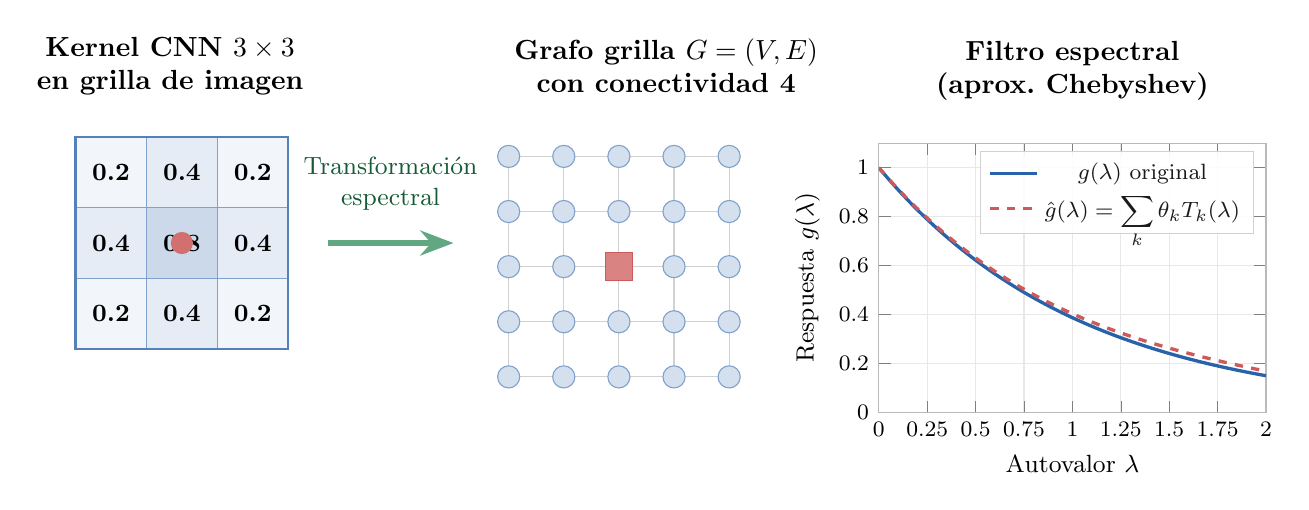
\begin{tikzpicture}[>=Stealth]

% ============================================================
% LEFT PANEL: Kernel CNN 3x3
% ============================================================

% Title
\node[font=\bfseries, align=center, text=black] at (1.2, 3.6)
  {Kernel CNN $3\times 3$\\en grilla de imagen};

% Kernel values (row, col) -> value
% Row 0 (top): 0.2, 0.4, 0.2
% Row 1 (mid): 0.4, 0.8, 0.4
% Row 2 (bot): 0.2, 0.4, 0.2

% Cell size
\def\cs{0.9}

% Draw filled cells with intensity proportional to value
% val=0.2 -> gdlblue!6, val=0.4 -> gdlblue!12, val=0.8 -> gdlblue!24
\foreach \row/\vals in {0/{0.2,0.4,0.2}, 1/{0.4,0.8,0.4}, 2/{0.2,0.4,0.2}} {
  \foreach \col [count=\ci from 0] in \vals {
    \pgfmathsetmacro{\fillint}{\col*30}
    \pgfmathsetmacro{\cx}{\ci*\cs + \cs/2}
    \pgfmathsetmacro{\cy}{(2-\row)*\cs + \cs/2}
    \fill[gdlblue!\fillint] (\cx, \cy) +(-\cs/2,-\cs/2) rectangle +(\cs/2,\cs/2);
    \draw[gdlblue!60] (\cx, \cy) +(-\cs/2,-\cs/2) rectangle +(\cs/2,\cs/2);
    \node[font=\bfseries\small] at (\cx, \cy) {\col};
  }
}

% Outer border
\draw[gdlblue!80, thick] (0, 0) rectangle (3*\cs, 3*\cs);

% Red dot on center cell (row=1, col=1)
\fill[gdlred!70] (1.5*\cs, 1.5*\cs) circle (4pt);

% ============================================================
% ARROW: Transformacion espectral
% ============================================================

\draw[->, gdlgreen!70, line width=2pt] (3.2, 1.35) -- (4.8, 1.35);
\node[font=\small, align=center, text=gdlgreen!70!black] at (4.0, 2.1)
  {Transformaci\'{o}n\\espectral};

% ============================================================
% MIDDLE PANEL: Grafo grilla 5x5
% ============================================================

% Title
\node[font=\bfseries, align=center, text=black] at (7.5, 3.6)
  {Grafo grilla $G = (V, E)$\\con conectividad 4};

% Grid parameters
\def\gs{0.7}   % grid spacing
\def\nr{5}     % number of rows/cols
\def\nsize{4pt} % node radius

% Origin for graph grid
\def\gox{5.5}
\def\goy{-0.35}

% Draw edges first (4-connectivity)
\foreach \r in {0,...,4} {
  \foreach \c in {0,...,4} {
    % Horizontal edge to the right
    \pgfmathtruncatemacro{\cnext}{\c+1}
    \ifnum\cnext<5
      \draw[gdlgray!40] (\gox+\c*\gs, \goy+\r*\gs) -- (\gox+\cnext*\gs, \goy+\r*\gs);
    \fi
    % Vertical edge upward
    \pgfmathtruncatemacro{\rnext}{\r+1}
    \ifnum\rnext<5
      \draw[gdlgray!40] (\gox+\c*\gs, \goy+\r*\gs) -- (\gox+\c*\gs, \goy+\rnext*\gs);
    \fi
  }
}

% Draw nodes
\foreach \r in {0,...,4} {
  \foreach \c in {0,...,4} {
    \pgfmathtruncatemacro{\iscenter}{(\r==2 && \c==2) ? 1 : 0}
    \ifnum\iscenter=1
      % Center node: red square
      \node[fill=gdlred!60, draw=gdlred!80, minimum size=10pt, inner sep=0pt]
        at (\gox+\c*\gs, \goy+\r*\gs) {};
    \else
      % Regular node: blue circle
      \fill[gdlblue!20] (\gox+\c*\gs, \goy+\r*\gs) circle (\nsize);
      \draw[gdlblue!60] (\gox+\c*\gs, \goy+\r*\gs) circle (\nsize);
    \fi
  }
}

% ============================================================
% RIGHT PANEL: Filtro espectral (pgfplots)
% ============================================================

\begin{axis}[
  at={(10.2cm, -0.8cm)},
  anchor=south west,
  width=6.5cm,
  height=5cm,
  title={\textbf{\begin{tabular}{c}Filtro espectral\\(aprox.\ Chebyshev)\end{tabular}}},
  title style={align=center, at={(0.5,1.05)}},
  xlabel={Autovalor $\lambda$},
  ylabel={Respuesta $g(\lambda)$},
  xmin=0, xmax=2,
  ymin=0, ymax=1.1,
  xtick={0, 0.25, 0.50, 0.75, 1.00, 1.25, 1.50, 1.75, 2.00},
  ytick={0, 0.2, 0.4, 0.6, 0.8, 1.0},
  grid=both,
  grid style={gdlgray!20},
  axis line style={gdlgray!60},
  tick label style={font=\footnotesize},
  label style={font=\small},
  legend pos=north east,
  legend style={font=\footnotesize, draw=gdlgray!40, fill=white, fill opacity=0.9},
  every axis plot/.append style={thick},
  samples=100,
  domain=0:2,
  clip=true,
]

% Original filter g(lambda) — smooth decreasing curve
\addplot[gdlblue, solid, line width=1.2pt]
  {exp(-0.95*x)};
\addlegendentry{$g(\lambda)$ original}

% Chebyshev approximation — very close to original, slight visible deviation
% Degree-4 Chebyshev fit to exp(-0.95x) on [0,2], with small deliberate offset
\addplot[gdlred!80, dashed, line width=1.2pt]
  {1 - 0.92*x + 0.41*x^2 - 0.095*x^3 + 0.008*x^4};
\addlegendentry{$\hat{g}(\lambda) = \displaystyle\sum_k \theta_k T_k(\lambda)$}

\end{axis}

\end{tikzpicture}
\end{document}
